\section{样本及抽样分布}
\subsection{随机样本}

\begin{definition}
    设$X$是具有分布函数$F$的随机变量,若$X_1,X_2,\cdots,X_n$是具有同一分布函数$F$的、相互独立的随机变量,则称$X_1,X_2,\cdots,X_n$为从分布
    函数$F$(或总体$F$、或总体$X$)得到的{\heiti 容量为$n$的简单随机样本},简称{\heiti 样本},它们的观察值$x_1,x_2,\cdots,x_n$称为
    {\heiti 样本值},又称为$X$的$n$个{\heiti 独立的观察值}。

    由定义得:若$X_1,X_2,\cdots,X_n$为$F$的一个样本,则$X_1,X_2,\cdots,X_n$相互独立,且它们的分布函数都是$F$,所以$(X_1,X_2,\cdots,X_n)$
    的分布函数为
    $$F^\ast(x_1,x_2,\cdots,x_n)=\prod _{i=1}^n F(x_i)$$
    又若$X$具有概率密度$f$,则$(X_1,X_2,\cdots,X_n)$的概率密度为
    $$f^\ast(x_1,x_2,\cdots,x_n)=\prod _{i=1}^n f(x_i)$$
\end{definition}

\subsection{直方图和箱线图}
直方图和箱线图的定义及画法略。

\subsection{抽样分布}
\begin{definition}
    \begin{definition}
        设$X_1,X_2,\cdots,X_n$是来自总体$X$的一个样本,$g(X_1,X_2,\cdots,X_n)$是
        $X_1,X_2,\cdots,X_n$的函数,若$g$中不含未知参数,则称$g(X_1,X_2,\cdots,X_n)$
        是一{\heiti 统计量}。

        因为$X_1,X_2,\cdots,X_n$都是随机变量,而统计量$g(X_1,X_2,\cdots,X_n)$是随机变量的函数,因此统计量是一个随机变量.
        设$x_1,x_2,\cdots,x_n$是相应于样本$X_1,X_2,\cdots,X_n$的样本值,则称$g(x_1,x_2,\cdots,x_n)$是$g(X_1,X_2,\cdots,X_n)$的观察值。

        下面列出几个常用的统计量,设$X_1,X_2,\cdots,X_n$是来自总体$X$的一个样本,$x_1,x_2,\cdots,x_n$是这一样本的观察值,定义

        {\heiti 样本平均值} $$\overline{X}=\frac{1}{n}\sum_{i=1}^nX_i$$

        {\heiti 样本方差}$$S^2=\frac{1}{n-1}\sum_{i=1}^n{(X_i-\overline{X})}^2=\frac{1}{n-1}(\sum_{i=1}^nX_i^2-n\overline{X}^2)$$

        {\heiti 样本标准差}$$S=\sqrt{S^2}=\sqrt{\frac{1}{n-1}\sum_{i=1}^n{(X_i-\overline{X})}^2}$$

        {\heiti 样本$k$阶(原点)矩}$$A_k=\frac{1}{n}\sum_{i=1}^nX_i^k,\quad k=1,2,\cdots$$

        {\heiti 样本$k$阶中心矩}$$B_k=\frac{1}{n}\sum_{i=1}^n{(X_i-\overline{X})}^k,\quad k=2,3,\cdots$$\\
        它们的观察值分别为
        $$\overline{x}=\frac{1}{n}\sum_{i=1}^nx_i$$
        $$s^2=\frac{1}{n-1}\sum_{i=1}^n{(x_i-\overline{x})}^2=\frac{1}{n-1}(\sum_{i=1}^nx_i^2-n\overline{x}^2)$$
        $$s=\sqrt{\frac{1}{n-1}\sum_{i=1}^n{(x_i-\overline{x})}^2}$$
        $$a_k=\frac{1}{n}\sum_{i=1}^nx_i^k,\quad k=1,2,\cdots$$
        $$b_k=\frac{1}{n}\sum_{i=1}^n{(x_i-\overline{x})}^k,\quad k=2,3,\cdots$$
    \end{definition}
\end{definition}

\begin{definition}[经验分布函数]
    与总体分布函数$F(x)$相应的统计量——经验分布函数的做法为:
    设$X_1,X_2,\cdots,X_n$是总体$F$的一个样本,用$S(x),-\infty<x<\infty$表示$X_1,X_2,\cdots,X_n$
    中不大于$x$的随机变量的个数.定义经验分布函数$F_n(x)$为
    $$F_n(x)=\frac{1}{n}S(x),-\infty<x<\infty$$
\end{definition}

\begin{definition}[$\chi^2$分布]
    设$X_1,X_2,\cdots,X_n$是来自总体$N(0,1)$的样本,则称统计量
    $$\chi^2=X_1^2+X_2^2+\cdots+X_n^2$$
    服从自由度为$n$的{\heiti $\chi^2$分布},记为$\chi^2\sim \chi^2(n)$.此处自由度是指上式右端包含的独立变量的个数。
    \begin{figure}[H]
        \centering
        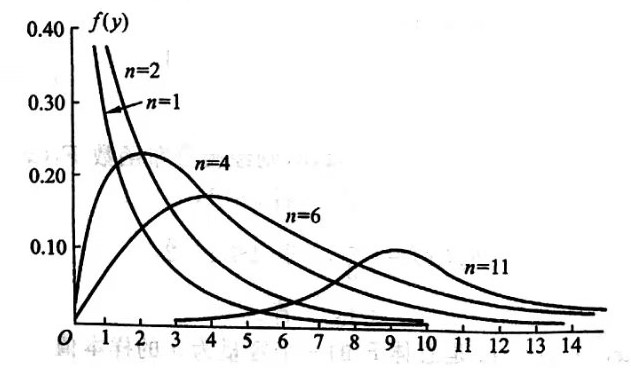
\includegraphics[scale=0.4]{1.jpg}
        \caption{$\chi^2(n)$分布的概率密度图}
    \end{figure} 
    $\chi^2(n)$分布的概率密度为
    $$f(y)=\left\{\begin{array}{ll}
        \frac{1}{2^{n/2}\Gamma (n/2)}y^{n/2-1}e^{-y/2},& y>0\\
        0,&\mbox{其他}
    \end{array}\right.$$
    $f(y)$的图形如图1所示。

\end{definition}

\begin{theorem}
    $\chi^2$分布的性质:

    {\heiti $\chi^2$分布的可加性}$\quad$ 设$\chi^2_1\sim \chi^2(n_1),\chi^2_2\sim \chi^2(n_2)$,并且
    $\chi^2_1,\chi^2_2$相互独立,则有
    $$\chi^2_1+\chi^2_2\sim \chi^2(n_1+n_2)$$

    {\heiti $\chi^2$分布的数学期望和方差}$\quad$ 若$\chi^2\sim \chi^2(n)$,则有
    $$E(\chi^2)=n,\quad D(\chi^2)=2n$$
    
    {\heiti $\chi^2$分布的上分位点}$\quad$ 对于给定的正数$\alpha,0<\alpha<1$,满足条件
    $$P\{\chi^2>\chi_\alpha^2(n)\}=\int_{\chi_\alpha^2(n)}^\infty f(y)\,dy=\alpha$$
    的点$\chi_\alpha^2(n)$就是$\chi^2(n)$分布的上$\alpha$分位点。

\end{theorem}